%% Trabalho final de PSI0325 — template SBrT 2026 (sbrt.cls)
\documentclass{sbrt}
\usepackage[english,brazil]{babel}
\usepackage[utf8]{inputenc}
\usepackage{graphicx}
\usepackage{amsmath}

\begin{document}

\title{Identificação de espécies de morcegos pelo pulso de ecolocalização com uma rede MLP}

\author{Victor Emanuel Ramos de Carvalho
\thanks{Victor Emanuel Ramos de Carvalho, Escola Politécnica, Universidade de São Paulo, São Paulo-SP, e-mail: victor\_carvalho@usp.br. Trabalho final da disciplina PSI0325 -- Fundamentos de Adaptação e Aprendizado de Máquina.}%
}

\maketitle

\markboth{PSI0325 -- TRABALHO FINAL -- ESCOLA POLITÉCNICA DA USP -- OUTUBRO DE 2026}{}

\begin{resumo}
Este trabalho treina uma rede MLP para identificar 8 espécies de morcegos a partir de cinco medidas do pulso de ecolocalização, em 13.408 gravações identificadas por especialistas. A rede tem uma camada oculta de 8 neurônios e é treinada com entropia cruzada ponderada pela frequência das classes. No conjunto de teste, a acurácia balanceada é 0,959, contra 0,942 de um modelo linear e 0,697 de uma regra baseada na chave de identificação. Os erros se concentram em espécies do mesmo gênero. Checagens com rótulos embaralhados e com locais fora do treino indicam que o resultado não decorre de vazamento.
\end{resumo}
\begin{chave}
Rede neural MLP, bioacústica, classificação multiclasse, morcegos.
\end{chave}

\begin{abstract}
This work trains an MLP network to identify 8 bat species from five measurements of the echolocation pulse, using 13,408 recordings labeled by experts. The network has one hidden layer with 8 neurons and is trained with cross-entropy weighted by class frequency. On the test set, its balanced accuracy is 0.959, against 0.942 for a linear model and 0.697 for a rule based on the identification key. Errors concentrate on species of the same genus. Checks with shuffled labels and with held-out recording sites indicate that the result is not due to leakage.
\end{abstract}
\begin{keywords}
MLP neural network, bioacoustics, multiclass classification, bats.
\end{keywords}

\section{Introdução}

No monitoramento acústico de morcegos, detectores gravam os pulsos de ecolocalização e especialistas identificam a espécie de cada gravação olhando o sonograma e medindo o pulso. É um trabalho manual, que limita o número de gravações analisadas. Este trabalho trata a etapa final dessa identificação como um problema de classificação: dado o vetor de medidas de uma gravação, prever a espécie que a emitiu. A extração das medidas a partir do áudio já foi feita na base e não faz parte do escopo.

A chave de identificação usada pelos especialistas atribui faixas de frequência sobrepostas a espécies diferentes e as separa por critérios adicionais, como a duração do pulso. Um critério que vale numa faixa não vale em outra, o que sugere fronteiras de decisão não lineares e motiva o uso de uma rede MLP, com a regressão logística como referência linear.

O trabalho seguiu uma progressão: primeiro um problema binário (\textit{Myotis lavali} contra as demais espécies), depois um par difícil e desbalanceado (\textit{M. lavali} contra \textit{Molossops temminckii}) e, por fim, o problema com 8 espécies, adicionando uma de cada vez. Todo o código foi escrito em PyTorch~\cite{pytorch}; divisão dos dados, normalização e métricas foram implementadas em NumPy a partir das fórmulas da disciplina~\cite{psi0325}.

\section{Base de dados}

A base reúne gravações de dois projetos de monitoramento no norte de Minas Gerais, em parques urbanos de Montes Claros e no Parque Estadual da Lapa Grande, feitas com detectores SM2BAT a 768~kHz entre 2024 e 2026 e identificadas por especialistas~\cite{base}. Os dados pertencem ao Centro de Bioacústica do Norte de Minas Gerais e não são públicos. São 14.540 gravações de 23 espécies ou sonótipos; as 15 categorias com menos de 379 gravações somam 1.053 gravações (7,3\%) e ficaram de fora do recorte.

\subsection{Recorte e limpeza}

Foram mantidas as 8 espécies com pelo menos 379 gravações; o sonótipo \textit{Molossidae1} (identificado só até família) foi excluído. Cinco gravações com erro grave foram removidas (\textit{M. lavali} com frequência de maior energia abaixo de 10~kHz e \textit{Eumops} sp. acima de 45~kHz) e, de 27 duplicatas exatas, manteve-se uma cópia. Gravações com duas espécies têm uma linha por espécie e foram mantidas. Restam 13.408 gravações (Tabela~\ref{tab:dados}), com razão de 19 para 1 entre a espécie mais e a menos frequente.

\begin{table}[htb]
\caption{\label{tab:dados}Gravações por espécie e divisão estratificada.}
\begin{center}
\begin{tabular}{lrrrr}\hline
Espécie & Total & Treino & Valid. & Teste\\\hline
\textit{Myotis lavali} & 7.284 & 5.099 & 1.093 & 1.092\\
\textit{Molossus molossus} & 1.648 & 1.154 & 247 & 247\\
\textit{Lasiurus blossevillii} & 1.082 & 757 & 162 & 163\\
\textit{Neoeptesicus furinalis} & 1.014 & 710 & 152 & 152\\
\textit{Eumops} sp. & 723 & 506 & 108 & 109\\
\textit{Molossus currentium} & 716 & 501 & 107 & 108\\
\textit{Molossops temminckii} & 557 & 390 & 84 & 83\\
\textit{Myotis nigricans} & 384 & 269 & 58 & 57\\\hline
Total & 13.408 & 9.386 & 2.011 & 2.011\\\hline
\end{tabular}
\end{center}
\end{table}

\subsection{Entradas da rede}

Cada gravação é descrita por cinco medidas médias do pulso: frequência mínima (Fmin), frequência máxima (Fmax), largura de banda, frequência de maior energia (FME) e duração. A largura de banda foi recalculada como $\mathrm{Fmax}-\mathrm{Fmin}$, pois a coluna original não confere com essa diferença em cerca de 8,5\% dos pulsos medidos.

Colunas da planilha foram excluídas por três motivos. \textit{Tipo de pulso}, família, gênero e subfamília são fórmulas da planilha calculadas a partir do nome da espécie; usá-las seria entregar o rótulo como entrada (sozinho, o tipo de pulso separa \textit{M. lavali} de \textit{M. temminckii} com coeficiente de Matthews~\cite{matthews} igual a 1,00). As colunas \textit{Fstart} e \textit{Fend} estão em segundos, ou seja, indicam a posição do pulso na gravação e não uma propriedade do chamado. Local, data e gravador descrevem onde e quando se gravou, não o pulso.

\subsection{Divisão e normalização}

A divisão é estratificada por espécie, 70\% para treino, 15\% para validação e 15\% para teste, com semente 42. O treino ajusta os pesos, a validação escolhe a época e os hiperparâmetros, e o teste foi usado uma única vez, ao final. Cada atributo $x_j$ é normalizado para média zero e variância unitária,
\begin{equation}
\tilde{x}_j=\frac{x_j-\mu_j}{\sigma_j},
\end{equation}
com $\mu_j$ e $\sigma_j$ calculados apenas no treino. A análise exploratória (histogramas, PCA e LDA) e a remoção dos cinco erros graves foram feitas na base inteira, antes da divisão; nenhum parâmetro de modelo foi ajustado nessa fase.

\section{Modelo e treinamento}

\subsection{Arquitetura e função custo}

A rede recebe as 5 entradas normalizadas, tem uma camada oculta de 8 neurônios com ativação tangente hiperbólica e uma camada de saída com $N_L=8$ neurônios, um por espécie. A saída passa pela função \textit{softmax},
\begin{equation}
y_k=\frac{e^{v_k}}{\sum_{\ell=1}^{N_L}e^{v_\ell}},
\end{equation}
em que $v_k$ é o campo local induzido do $k$-ésimo neurônio de saída, e a espécie prevista é a de maior $y_k$. A função custo é a entropia cruzada categórica, com cada exemplo ponderado pelo inverso da frequência da sua classe:
\begin{equation}
J=-\frac{1}{\sum_n w_{c(n)}}\sum_{n}w_{c(n)}\ln y_{c(n)}(n),\qquad w_c=\frac{N}{N_L\,N_c},
\end{equation}
em que $c(n)$ é a espécie do exemplo $n$, $N$ é o número de exemplos de treino e $N_c$ o número de exemplos da espécie $c$. Os pesos vão de 0,23 (\textit{M. lavali}) a 4,36 (\textit{M. nigricans}): errar uma espécie rara custa mais. Essa normalização pela soma dos pesos é a do \texttt{CrossEntropyLoss} do PyTorch; ela difere do fator $1/N_L$ da definição da disciplina apenas por uma constante, o que equivale a ajustar o passo.

\subsection{Otimização}

Os pesos são ajustados pelo Adam~\cite{adam} com passo 0,01, em mini-batches de 64 exemplos, por até 1000 épocas. A cada época calcula-se a perda na validação e guardam-se os pesos da época de menor perda. A Tabela~\ref{tab:config} resume o necessário para reproduzir o treino.

\begin{table}[htb]
\caption{\label{tab:config}Configuração do modelo final.}
\begin{center}
\begin{tabular}{ll}\hline
Entradas & 5 medidas, média 0 e variância 1 (treino)\\
Camada oculta & 1, com 8 neurônios, $\tanh$\\
Saída & 8 neurônios, \textit{softmax}\\
Inicialização & padrão do PyTorch, $\mathcal{U}(\pm 1/\sqrt{N_{j-1}})$\\
Função custo & entropia cruzada com peso $w_c$\\
Otimizador & Adam, passo 0,01\\
Mini-batch & 64, embaralhado a cada época\\
Épocas & até 1000; pesos do mínimo da validação\\
Regularização & nenhuma (sem \textit{dropout} e sem $\ell_2$)\\
Sementes & divisão: 42; treino: 0, 1 e 2\\
Software & Python 3.13, PyTorch 2.14 (CPU)\\\hline
\end{tabular}
\end{center}
\end{table}

\subsection{Escolha dos hiperparâmetros}

Partindo dessa configuração, variou-se um fator por vez, com três sementes cada, e uma mudança só seria adotada se aumentasse a acurácia balanceada média na validação em mais de 0,005, valor próximo do desvio observado entre sementes. A regra foi fixada antes dos experimentos. A Tabela~\ref{tab:hiper} mostra o resultado: nenhuma das 22 configurações passou do limiar, e todas ficaram entre 0,951 e 0,968. Mantiveram-se a rede menor e as opções mais simples.

\begin{table}[htb]
\caption{\label{tab:hiper}Acurácia balanceada na validação (média de 3 sementes). Configuração escolhida: 0,966.}
\begin{center}
\begin{tabular}{ll}\hline
Variação & Acurácia balanceada\\\hline
16, 32, 64 neurônios & 0,966; 0,964; 0,962\\
2 camadas ocultas & 0,964\\
ReLU; ReLU com inicialização de He~\cite{he} & 0,960; 0,961\\
Inicialização de Xavier; Glorot~\cite{glorot}; He & 0,968; 0,967; 0,966\\
SGD; SGD com momento; RMSprop & 0,966; 0,966; 0,966\\
Passo 0,001; 0,1 & 0,964; 0,965\\
\textit{Dropout}~\cite{dropout} 0,2; 0,5 & 0,965; 0,951\\
Regularização $\ell_2$ ($10^{-4}$) & 0,967\\
Mini-batch 32; 128 & 0,963; 0,964\\
64 neurônios com \textit{dropout} 0,2 & 0,966\\
Glorot com SGD e momento & 0,967\\\hline
\end{tabular}
\end{center}
\end{table}

O platô indica que, com estas cinco medidas, o desempenho é limitado pela sobreposição entre espécies, e não pela capacidade da rede. Com 64 neurônios, a perda de treino continua caindo enquanto a de validação sobe de 0,142 (época 98) para 0,195 (época 1000), um sinal de sobreajuste que a escolha dos pesos pelo mínimo da validação neutraliza. Com 8 neurônios, as duas curvas permanecem juntas (Fig.~\ref{fig:curvas}).

\begin{figure}[htb]
\begin{center}
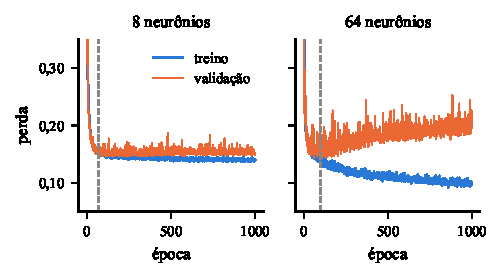
\includegraphics[width=\columnwidth]{figuras/curvas_8_64.pdf}
\end{center}
\caption{\label{fig:curvas}Perda (entropia cruzada com peso) de treino e de validação com 8 e 64 neurônios na camada oculta (semente 0). A linha tracejada marca a época de menor perda de validação, cujos pesos são guardados.}
\end{figure}

\section{Avaliação}

\subsection{Métricas}

Nos problemas binários iniciais usou-se o coeficiente de Matthews~\cite{matthews}, que resume a matriz de confusão $2\times 2$ num único número; no problema com 8 espécies, as métricas partem da matriz $8\times 8$. Para cada espécie, tratada como positiva, calculam-se a sensibilidade $S_c$ (fração das gravações da espécie que o modelo identifica) e a precisão $P_c$ (fração das previsões da espécie que estão corretas). A métrica principal é a acurácia balanceada,
\begin{equation}
\mathrm{AB}=\frac{1}{N_L}\sum_{c=1}^{N_L}S_c,
\end{equation}
em que cada espécie tem o mesmo peso; com classes desbalanceadas, a acurácia comum seria dominada por \textit{M. lavali}. Reportam-se também o F1 macro~\cite{grandini}, média de $F1_c=2P_cS_c/(P_c+S_c)$, e a acurácia.

Duas referências são avaliadas no mesmo conjunto: um modelo linear (regressão \textit{softmax}, sem camada oculta), com a mesma função custo, mini-batch e sementes, e otimizador escolhido na validação entre cinco opções (Adam com passo 0,01 e até 1000 épocas, o mesmo regime da MLP) e uma regra sem aprendizado que atribui a espécie cuja FME típica na chave de identificação, convertida pelo ponto médio de cada faixa, está mais próxima da FME medida.

\subsection{Progressão até 8 espécies}

Nos problemas iniciais (validação, uma semente), a MLP superou o modelo linear: em \textit{M. lavali} contra as demais, com o mesmo otimizador para os dois (SGD, passo 0,1, 400 épocas), o coeficiente de Matthews passou de 0,884 para 0,968 e os falsos positivos de 102 para 17, a maioria de \textit{M. nigricans}. No par \textit{M. lavali} e \textit{M. temminckii}, as duas espécies têm FME de cerca de 50~kHz; uma MLP que recebe só a FME prevê sempre \textit{M. lavali} (coeficiente 0,000), enquanto com as cinco medidas chega a 0,963. A rede usa informação que a regra baseada na FME não usa.

O mesmo par, com razão de 13 para 1, serviu para comparar formas de tratar o desbalanceamento (Tabela~\ref{tab:desbal}; 84 \textit{M. temminckii} entre 1.177 gravações de validação, \textit{M. temminckii} como classe positiva). A subamostragem da classe majoritária, que descarta gravações de \textit{M. lavali} até igualar as classes no treino, reduziu a precisão e o coeficiente de Matthews; por isso, e por orientação do professor, não foi usada. O peso inverso à frequência eliminou os falsos negativos, mas aumentou os falsos positivos, uma troca que reaparece no problema com 8 espécies.

\begin{table}[htb]
\caption{\label{tab:desbal}Desbalanceamento no par \textit{M. lavali} e \textit{M. temminckii} (MLP, validação; sem correção: uma semente).}
\begin{center}
\begin{tabular}{lccc}\hline
Estratégia & Sensib. & Precisão & MCC\\\hline
Sem correção & 0,988 & 0,943 & 0,963\\
Subamostragem 1:1 (5 sorteios) & 0,986 & 0,889 & 0,931\\
Peso inverso (3 sementes) & 1,000 & 0,891 & 0,939\\\hline
\end{tabular}
\end{center}
\end{table}

A Fig.~\ref{fig:crescente} mostra o efeito de adicionar as espécies em ordem de frequência. Antes de rodar, definiu-se que haveria degradação se a espécie nova tivesse sensibilidade abaixo de 0,70 ou se a acurácia balanceada caísse mais de 5 pontos; isso não ocorreu. Com 8 espécies, o peso por classe elevou a acurácia balanceada de 0,947 para 0,969 e a sensibilidade de \textit{M. nigricans} de 0,836 para 0,988, ao custo de mais falsos positivos (F1 macro de 0,948 para 0,927). Como o objetivo é não perder espécies raras, a métrica principal é a acurácia balanceada, e por ela o peso é preferível; pelo F1 macro a escolha seria a oposta. Adotou-se o peso. A representação com os três pulsos de cada gravação (25 atributos) não superou a de médias (0,949 e 0,947, sem peso) e foi descartada.

\begin{figure}[htb]
\begin{center}
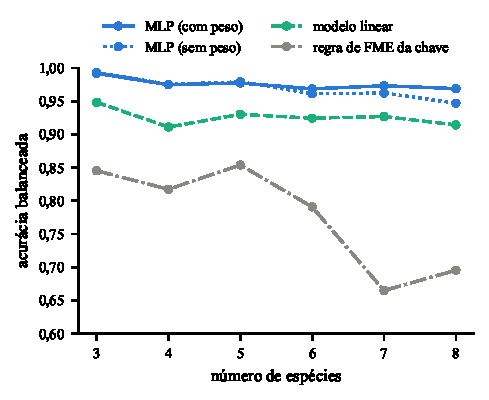
\includegraphics[width=\columnwidth]{figuras/curva_crescente.pdf}
\end{center}
\caption{\label{fig:crescente}Acurácia balanceada na validação ao adicionar uma espécie por vez (média de 3 sementes; modelo linear sem peso; 12.866 gravações com os três pulsos medidos).}
\end{figure}

\subsection{Resultado no teste}

A Tabela~\ref{tab:resultado} compara validação e teste. A queda de 0,966 para 0,959 é compatível com a escolha dos hiperparâmetros na validação. A MLP supera o modelo linear treinado nas mesmas condições, com cerca de 30\% a menos de erro em acurácia balanceada (4,1\% contra 5,8\%).

\begin{table}[htb]
\caption{\label{tab:resultado}Desempenho (média $\pm$ desvio de 3 sementes).}
\begin{center}
\begin{tabular}{llcc}\hline
Modelo & Métrica & Validação & Teste\\\hline
MLP & AB & 0,966 $\pm$ 0,002 & 0,959 $\pm$ $<$0,001\\
 & F1 macro & 0,922 $\pm$ 0,004 & 0,926 $\pm$ 0,005\\
 & Acurácia & 0,950 $\pm$ 0,003 & 0,955 $\pm$ 0,004\\\hline
Linear & AB & 0,953 $\pm$ 0,001 & 0,942 $\pm$ 0,001\\
 & F1 macro & 0,901 $\pm$ 0,002 & 0,901 $\pm$ 0,001\\\hline
Regra & AB & 0,694 & 0,697\\\hline
\end{tabular}
\end{center}
\end{table}

A Fig.~\ref{fig:matriz} detalha o teste. Todas as espécies têm sensibilidade acima de 0,92 (de 0,928 em \textit{M. molossus} a 0,996 em \textit{M. temminckii}), e a precisão fica acima de 0,89 em todas, exceto \textit{M. nigricans} (0,613): em média, 34 gravações de \textit{M. lavali}, do mesmo gênero e com faixas de frequência vizinhas, são classificadas como \textit{M. nigricans}. Esse é o custo do peso por classe. As demais confusões também ocorrem entre espécies próximas: \textit{Molossus molossus} e \textit{M. currentium}, \textit{Neoeptesicus furinalis} e \textit{Lasiurus blossevillii}.

\begin{figure}[htb]
\begin{center}
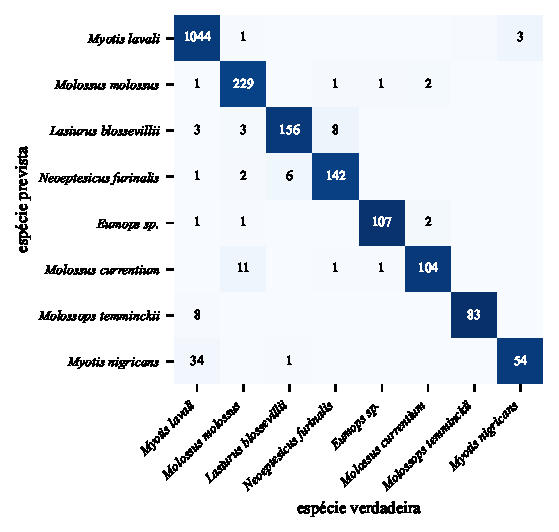
\includegraphics[width=\columnwidth]{figuras/matriz_teste.pdf}
\end{center}
\caption{\label{fig:matriz}Matriz de confusão da MLP no teste (média de 3 sementes).}
\end{figure}

\subsection{Checagens}

Como o desempenho é alto, explicações alternativas foram testadas sem usar o teste. Com os rótulos do treino embaralhados, o coeficiente de Matthews cai para valores entre $-0{,}020$ e 0,096: não há vazamento de informação na preparação. A regra baseada na FME da chave obtém acurácia balanceada de 0,694 com 8 espécies, bem abaixo da MLP: a rede não apenas reproduz a regra. Por fim, numa validação cruzada em que cada local de coleta fica fora do treino uma vez, a acurácia balanceada passa de 0,966 para 0,955; o que mais piora fora do local de origem é a precisão de \textit{M. nigricans} (0,572). Gravações feitas segundos depois no mesmo local costumam ser o mesmo animal: 54\% das gravações de teste têm uma assim no treino, mas a acurácia é 0,965 com e 0,955 sem essa vizinha, e numa divisão em que noites inteiras (local e data) ficam fora do treino a acurácia balanceada é 0,959. Por fim, espécie e projeto de origem estão associados (\textit{M. currentium} e \textit{M. nigricans} vêm quase só dos parques urbanos) e não podem ser separados; em \textit{M. molossus}, a FME média é de 34,5~kHz num projeto e 40,1~kHz no outro, o que sugere critérios de identificação diferentes.

\subsection{Validação externa}

Depois de o modelo estar congelado, a planilha original recebeu novas gravações. Numa cópia de 1º de outubro de 2026, 908 gravações das 8 espécies não constavam da base usada (nome de arquivo ausente e nenhum vetor de medidas idêntico); 796 delas são de noites (local e data) que não aparecem no treino. Sem nenhum ajuste, a MLP obteve acurácia de 0,958 nas 908 e de 0,962 nas 796, com acurácia balanceada de 0,930 e 0,953, contra 0,662 e 0,672 da regra da chave. As espécies mais representadas mantiveram sensibilidade alta (\textit{M. lavali}: 654 de 674; \textit{M. temminckii}: 122 de 128; \textit{N. furinalis}: 44 de 48; \textit{M. currentium}: 31 de 32); \textit{M. molossus} foi a exceção (12 de 19), com sete gravações classificadas como \textit{M. currentium}. \textit{Eumops} sp., \textit{L. blossevillii} e \textit{M. nigricans} tiveram de 1 a 4 gravações, poucas para conclusões por espécie.

\section{Conclusões}

Uma MLP com uma camada oculta de 8 neurônios identifica 8 espécies de morcegos a partir de cinco medidas do pulso com acurácia balanceada de 0,959 no teste, acima do modelo linear (0,942) e da regra de frequência da chave de identificação (0,697). O desempenho se manteve em gravações coletadas depois, em noites não usadas no treino (acurácia balanceada de 0,953). Redes maiores e outras escolhas de hiperparâmetros não melhoraram o resultado, que é limitado pela sobreposição entre espécies do mesmo gênero.

O resultado tem limites. O rótulo é a identificação acústica feita por especialistas, sem captura dos animais, então as métricas medem concordância com eles. As medidas foram extraídas manualmente do sonograma. O modelo conhece apenas 8 espécies, de uma região e de um tipo de gravador, e cerca de 1,2\% dos nomes de arquivo indicam espécie diferente do rótulo, o que sugere algum ruído de rotulagem. Há ainda 190 gravações com duas espécies, cujas linhas podem ter caído em conjuntos diferentes (2,3\% da validação e 1,7\% do teste). Espécie e projeto de origem estão associados, e os rótulos de \textit{M. molossus} parecem seguir critérios diferentes entre os projetos. As 15 espécies menos frequentes ficaram de fora: uma gravação de outra espécie será atribuída a uma das 8. Na prática, o modelo serve como triagem: raramente deixa de indicar uma espécie rara, mas as indicações de \textit{M. nigricans} precisam de conferência. Continuações naturais são extrair as medidas diretamente do áudio, incluir as espécies raras e permitir que o modelo recuse gravações de espécies que não conhece.

\begin{thebibliography}{99}
\bibitem{base} Centro de Bioacústica do Norte de Minas Gerais, dados de monitoramento acústico dos projetos Cidade Viva (Montes Claros-MG) e Parque Estadual da Lapa Grande, 2024--2026. Dados não publicados.
\bibitem{psi0325} PSI0325 -- Fundamentos de Adaptação e Aprendizado de Máquina, material de aula, Escola Politécnica da USP, 2026. Disponível em: https://psi0325.github.io.
\bibitem{pytorch} A. Paszke \textit{et al.}, ``PyTorch: An imperative style, high-performance deep learning library,'' em \textit{Advances in Neural Information Processing Systems 32}, 2019.
\bibitem{adam} D. P. Kingma e J. Ba, ``Adam: A method for stochastic optimization,'' em \textit{International Conference on Learning Representations}, 2015.
\bibitem{glorot} X. Glorot e Y. Bengio, ``Understanding the difficulty of training deep feedforward neural networks,'' em \textit{Proc. AISTATS}, pp. 249--256, 2010.
\bibitem{he} K. He, X. Zhang, S. Ren e J. Sun, ``Delving deep into rectifiers: Surpassing human-level performance on ImageNet classification,'' em \textit{Proc. IEEE ICCV}, pp. 1026--1034, 2015.
\bibitem{dropout} N. Srivastava, G. Hinton, A. Krizhevsky, I. Sutskever e R. Salakhutdinov, ``Dropout: A simple way to prevent neural networks from overfitting,'' \textit{Journal of Machine Learning Research}, v. 15, pp. 1929--1958, 2014.
\bibitem{matthews} B. W. Matthews, ``Comparison of the predicted and observed secondary structure of T4 phage lysozyme,'' \textit{Biochimica et Biophysica Acta}, v. 405, n. 2, pp. 442--451, 1975.
\bibitem{grandini} M. Grandini, E. Bagli e G. Visani, ``Metrics for multi-class classification: An overview,'' arXiv:2008.05756, 2020.
\end{thebibliography}

\end{document}
